\section{Results}
\label{sec:Results}
Plotting the probability of chaos against the competition parameter (see figure \ref{fig:Results}), we observe a clear maximum around $ \epsilon = 0 $. The likelihood of chaotic behaviour for neutral competition at the prey's trophic level is thus higher than for dominant inter or intraspecific competition. This result remains true for systems with a different number of species (figures \ref{fig:Results} and \ref{fig:Contour}).

The overall likelihood of chaos, which can be interpreted as the area under the curve in figure \ref{fig:Results}, increases with the size of the food web. This effect should not be surprising: the more dimensions the phase space has, the easier is to fulfill the requirements of the complex geometry of a chaotic attractor \citep{Strogatz1994}. Even in those higher dimensional cases, there is still a clear maximum at neutral competition. Another local maximum was observed for low values of $ \epsilon $, meaning that weak competitive coupling also promotes chaos in our model.

\begin{figure}
	\begin{center}
		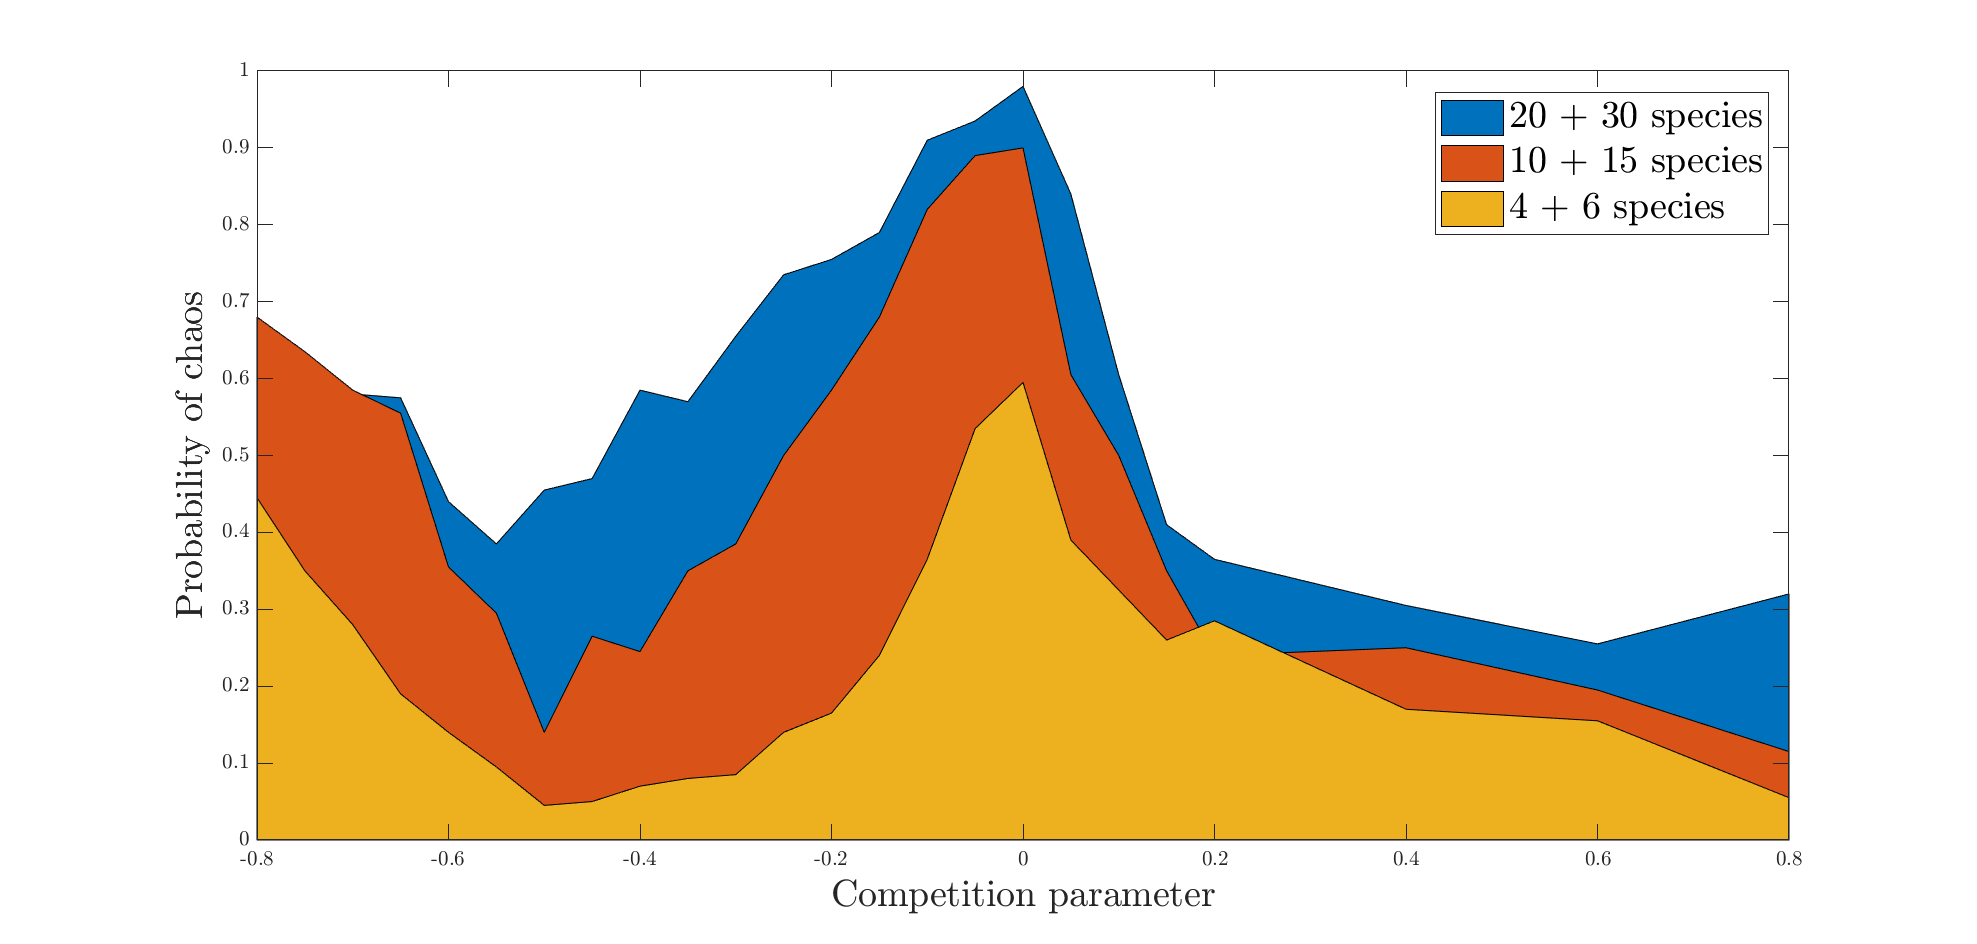
\includegraphics[width=1\columnwidth]{results.png}
	\end{center}
	\caption{Results for a low, medium and high dimensional system. The consumers' population is fixed as $ 2/3 $ of the prey's population. Notice how the probability of chaos has a local maximum around $\epsilon = 0$. The effect remains true for systems with different number of species. The overall probability of chaos, understood as the area under the curve, grows with the system size. }
	\label{fig:Results}
\end{figure}

\begin{figure}
	\begin{center}
		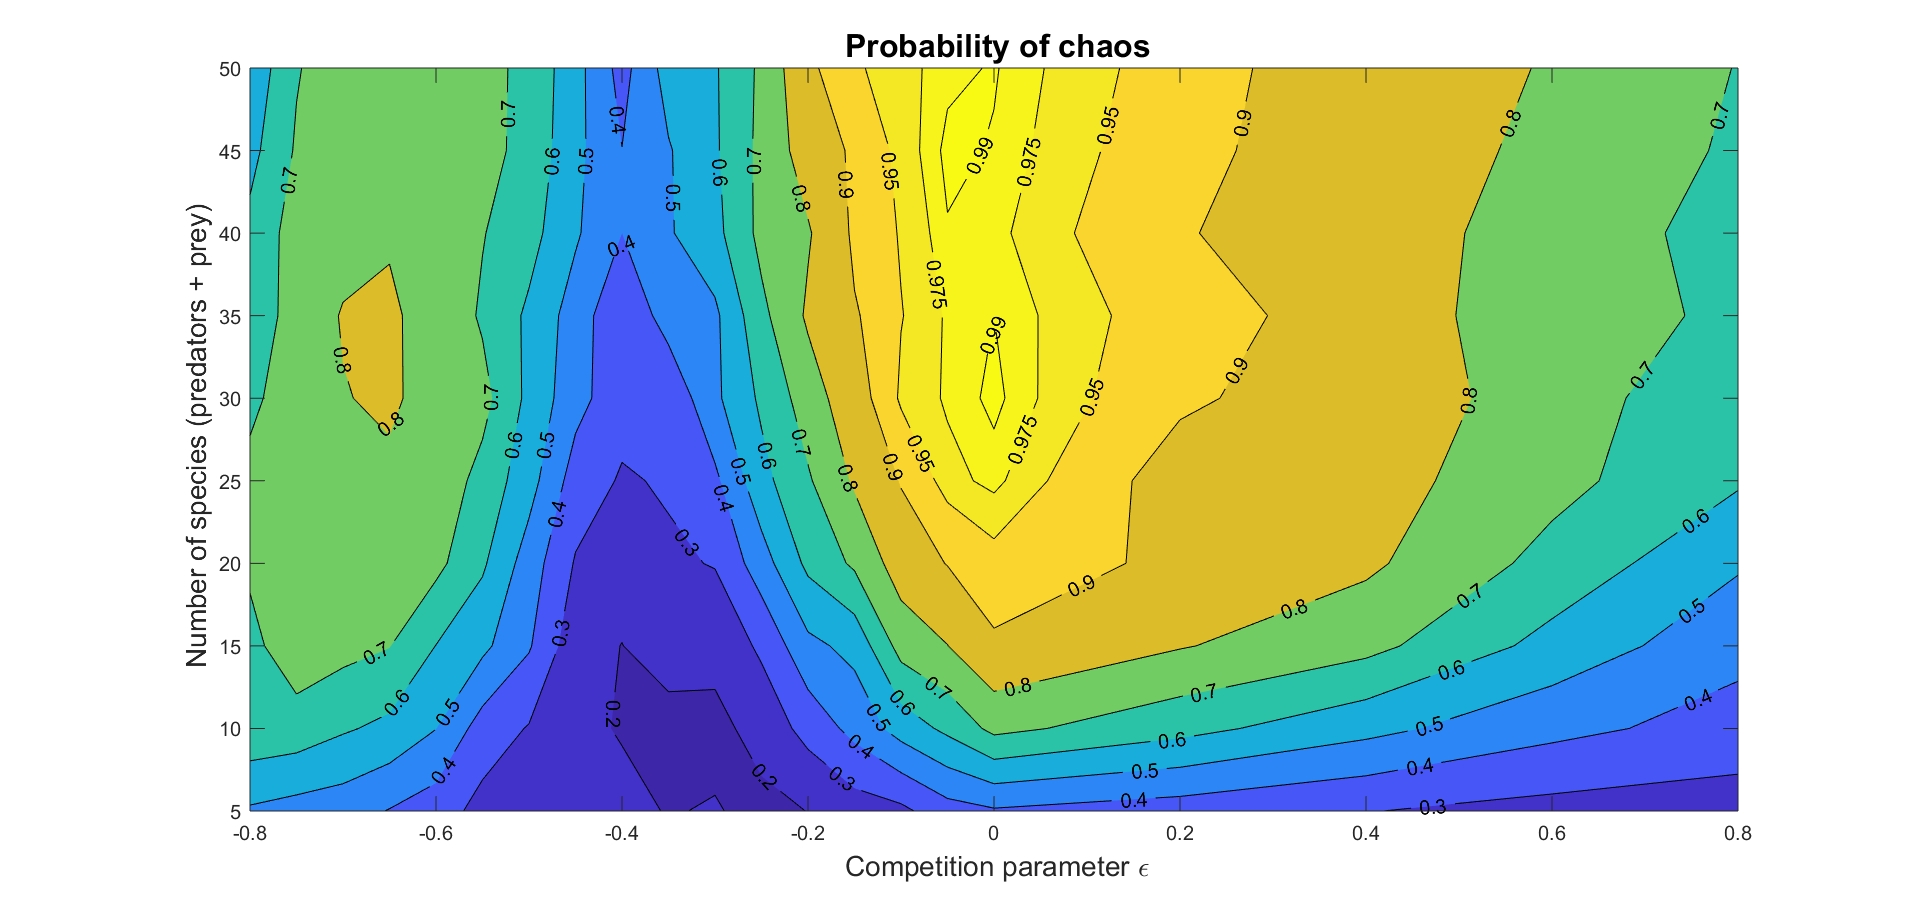
\includegraphics[width=1\columnwidth]{contour.png}
	\end{center}
	\caption{Contour map showing the probability of chaos for various competition parameters (horizontal axis) and number of species (vertical axis). The consumers' population is fixed as $ 2/3 $ of the prey's population. Notice that chaotic attractors appear more easily (i.e., for smaller systems) the closer is the competition to neutral (i.e., $ \epsilon = 0 $).}
	\label{fig:Contour}
\end{figure}